

\begin{frame}
\frametitle{Transient Response}
\begin{itemize}
\item The time response of a control system may be written as:
\begin{align*}
y(t) = y_{tr}(t) + y_{ss}(t)
\end {align*}
\\\item Where $y_{tr}(t)$ is the transient response and $y_{ss}(t)$ is the steady state response.
\item Most important characteristic of dynamic system is absolute stability.
\begin{itemize}
\item System is stable when returns to equilibrium if subject to initial condition
\item System is critically stable when oscillations of the output continue forever
\item System is unstable when output diverges without bound from equilibrium if subject to initial condition
\end{itemize}
\item Transient response: when input of system changes, output does not change immediately but takes time to go to steady state
\end{itemize}
\end{frame}

\begin{frame}
\frametitle{First-order systems}
\begin{itemize}
\item E.g.RC circuit, thermal system, ...
\vspace{0.25cm}
\\ 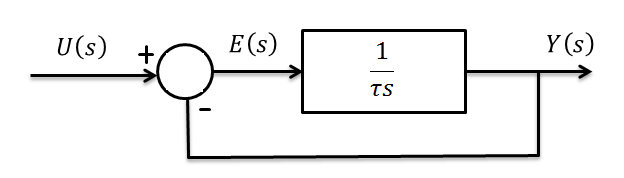
\includegraphics[width=0.7\linewidth]{Afbeelding1}
\vspace{0.5cm}
\item Transfer function is given by: $\frac{Y(s)}{U(s)} = \frac{1}{\tau s +1}$
\vspace{0.25cm}
\item Unit step response
\begin{itemize}
\vspace{0.25cm}
\item Laplace of unit-step is $\frac{1}{s}$ $\rightarrow$ substituting $U(s)= \frac{1}{s}$ \\
\vspace{0.25cm}
into equation $Y(s) = \frac{1}{s}\frac{1}{\tau s +1}$
\vspace{0.25cm}
\item Expanding into partial fractions gives
\vspace{0.25cm}
\\ $Y(s)= \frac{1}{s} - \frac{\tau}{\tau s +1} = \frac{1}{s} - \frac{1}{s+\frac{1}{\tau}}$
 \end{itemize}
\end{itemize}
\end{frame}

\begin{frame}
\frametitle{Unit step transient response}
\begin{itemize}
\item$Y(s)= \frac{1}{s} - \frac{\tau}{\tau s +1} = \frac{1}{s} - \frac{1}{s+\frac{1}{\tau}}$
\vspace{0.25cm}
\item Taking the inverse Laplace transform
\vspace{0.25cm}
\\ $y(t) = 1 - e^{-\frac{t}{\tau}}$, for $t\ge 0$ 
\vspace{0.25cm}
\item At $t=0$, the output $c(t)=0$
\vspace{0.25cm}
\item At $t=\tau$, the output $c(t)=0.632$, or $c(t)$ has reached $63.2\% $ 
\vspace{0.25cm} \\of it's total change $y(\tau)= 1 - e^{-1} = 0.632$
\vspace{0.25cm}
\item Slope at time $t=0$ is $\frac{1}{\tau}$
\vspace{0.25cm}
\\ $\frac{dy}{dt}|_{t=0} = \frac{1}{\tau}e^{-\frac{t}{\tau}}|_{t=0} = \frac{1}{\tau}$
\vspace{0.25cm}
\item Where $\tau$ is called the system's time constant
\end{itemize}
\end{frame}

\begin{frame}
\frametitle{Unit step transient response}
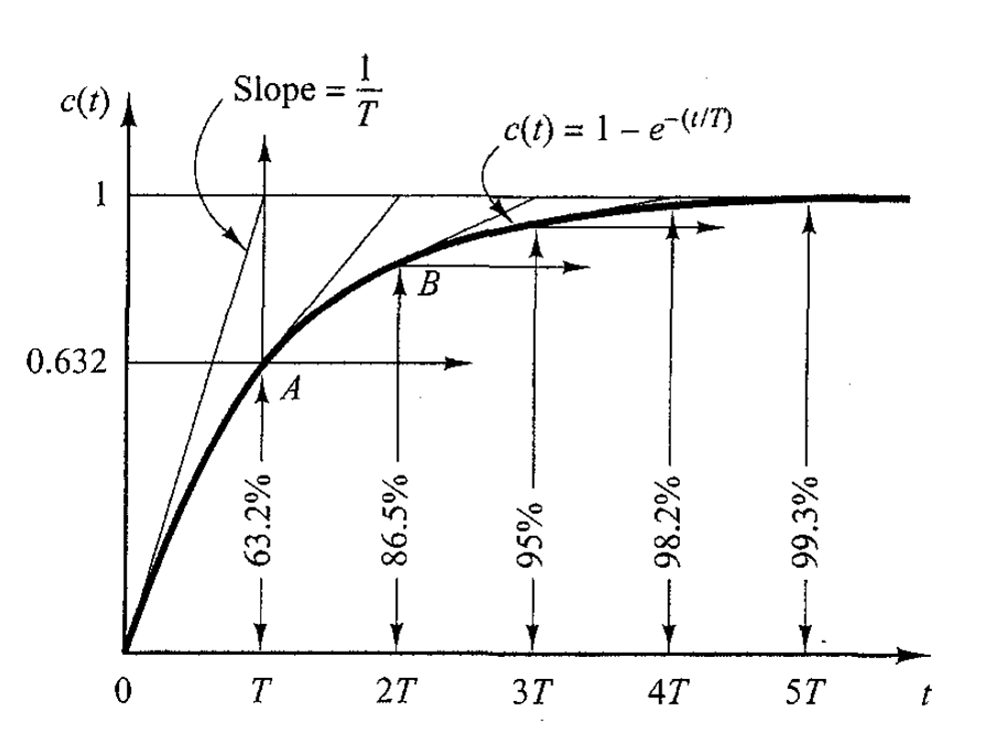
\includegraphics[width=1\linewidth]{Afbeelding2}
\end{frame}

\begin{frame}
\frametitle{Unit ramp transient response}
\begin{itemize}
\vspace{0.25cm}
\item Laplace transform of unit ramp is $\frac{1}{s^2}$
\vspace{0.25cm}
\\ $Y(s) = \frac{1}{\tau s +1} \frac{1}{s^2}$
\vspace{0.25cm}
\item Expanding into partial fractions gives
\vspace{0.25cm}
\\ $Y(s)= \frac{1}{s^2} - \frac{\tau}{s} + \frac{\tau^2}{\tau s +1}$
\vspace{0.25cm}
\item Taking the inverse Laplace transform 
\vspace{0.25cm}
\\ $y(t) = t -\tau + \tau e^{-\frac{t}{\tau}}$, for $t\ge 0$
\vspace{0.25cm}
\item The error signal $e(t)$ is then
\vspace{0.25cm}
\\ $e(t)=r(t) -c(t) = \tau(1-e^{-\frac{t}{\tau}})$
\vspace{0.25cm}
\item For $t$ approaching infinity, $e(t)$ approaches $\tau$
\vspace{0.25cm}
\\ $e(\infty) = \tau$
\end {itemize}
\end{frame}

\begin{frame}
\frametitle{Unit ramp transient response}
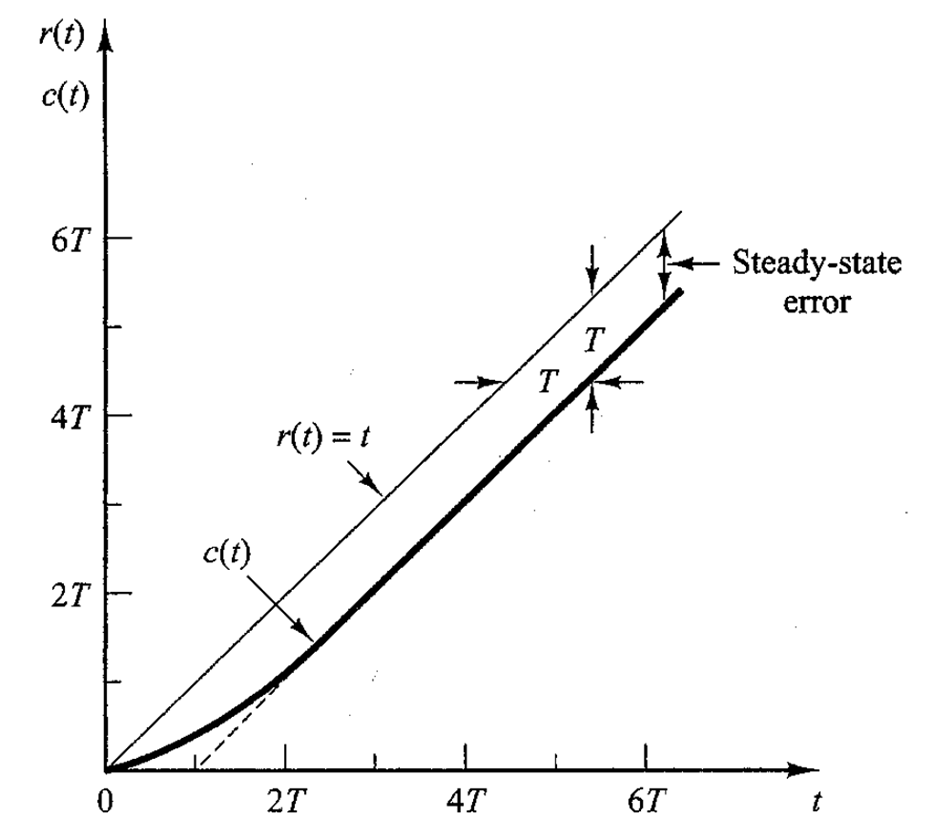
\includegraphics[width=0.8\linewidth]{Afbeelding4}
\end{frame}

\begin{frame}
\frametitle{Unit-Impulse Response}

\begin{itemize}
\item For a unit-impulse input, $U(s)=1$ and the output is
\vspace{0.2cm}
\\ 
\begin{align*}
Y(s)=\frac{1}{\tau s +1}
\end{align*}
\vspace{0.2cm}
\item The inverse Laplace transform gives
\vspace{0.2cm}
\\
\begin{align*}
y(t)= \frac{1}{\tau}e^{-\frac{t}{\tau}} ,\text{ for } t \ge 0
\end{align*}
\vspace{0.2cm}
\item For $t\rightarrow +\infty$, $y(t)\rightarrow 0$

\end{itemize}
\end{frame}

\begin{frame}
\frametitle{Unit-Impulse Response}
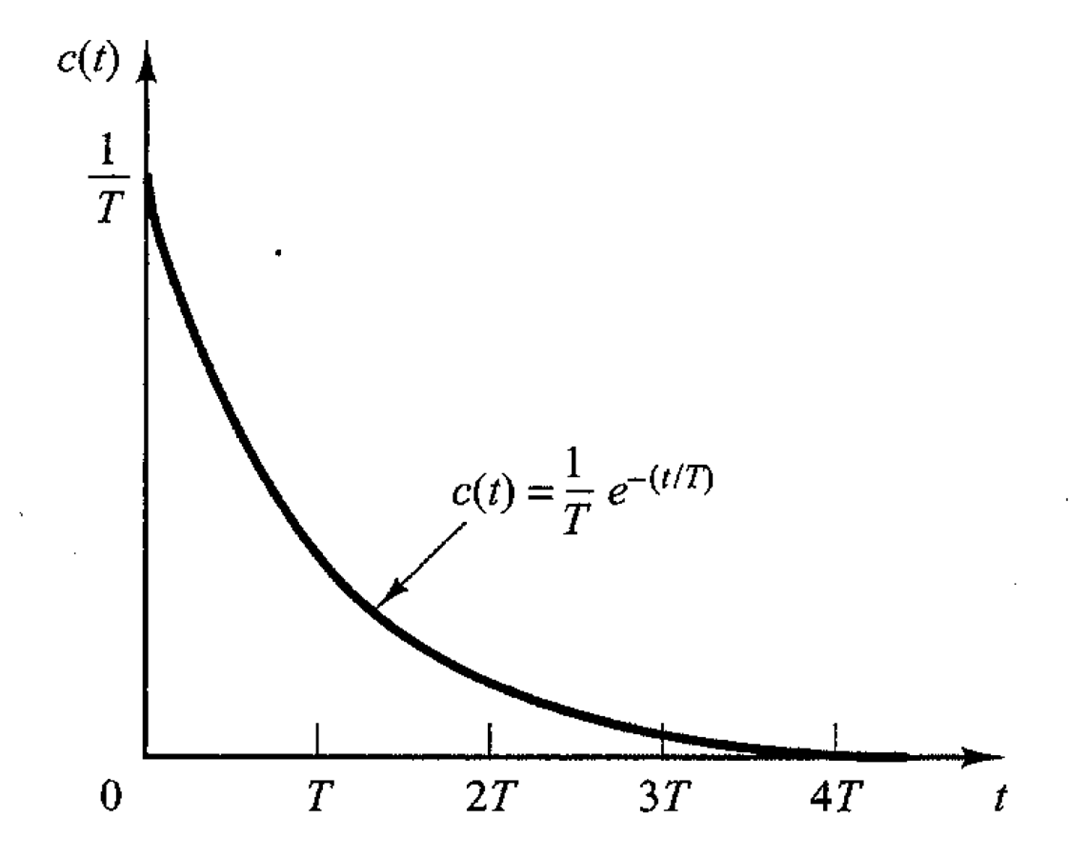
\includegraphics[width=0.8\linewidth]{Afbeelding5}
\end{frame}

\begin{frame}
\frametitle{Second order systems}
\begin{itemize}
\item A second order system can generally be written as:
\vspace{0.4cm}
\\ 
\begin{align*}
\frac{Y(s)}{U(s)}=H(s)=\frac{as^2+ bs+ c}{ds^2+ es+ f}
\end{align*}
\vspace{0.2cm}
\item A system where the closed-loop transfer function possesses two poles is called a second-order system
\vspace{0.4cm}
\item If the transfer function has two real poles, the frequency response can be found by combining the effects of both poles

\end{itemize}
\end{frame}

\begin{frame}
\begin{itemize} 
\vspace{-0.5cm}
\item Sometimes the transfer function has two complex conjugate poles. In that case we have to find a different solution for finding the frequency response.
\vspace{1cm}
\item In order to study the transient behaviour, let us first consider the following simplified example of a second order system
\\ 
\begin{align*}
H(s) = \frac{c}{ds^2+es+c}
\end {align*}
\vspace{-0.5cm}
\end{itemize}
\end{frame}

\begin{frame}
\frametitle{Step response second order system}
\begin{itemize}
\item $H(s) = \frac{c}{ds^2+es+c}$
\vspace{0.45cm}
\item The transfer function can be rewritten as:
\\ 
\begin{align*}
H(s) &= \frac{\frac{c}{d}}{s^2+\frac{e}{d}s+\frac{c}{d}}
\\ &= \frac{\frac{c}{d}}{[s+\frac{e}{2d}+\sqrt{(\frac{e}{2d})^2-\frac{c}{d}}][s+\frac{e}{2d}-\sqrt{(\frac{e}{2d})^2-\frac{c}{d}}]}
\end{align*}
\item The poles are complex conjugates if
\\ \vspace{-0.15cm}
\begin{align*}
e^2 -4dc <0
\end{align*}
\item The poles are real if
\\
\begin{align*}
e^2 -dc\ge 0
\end{align*}
\end{itemize}
\end{frame}

\begin{frame}
\frametitle{Step response second order system}
\begin{itemize}
\item To simplify the transient analysis, it is convenient to write
\\ 
\begin{align*}
\frac{f}{d} = \omega_n ^2\text{, } \frac{e}{d}=2\zeta\omega_n=2\sigma
\end{align*}
\item Where 
\\ $\sigma$ is het attenuation 
\\$\omega_n$ is the undamped natural frequency 
\\ $\zeta$ is the damping ratio
\vspace{0.25cm}
\item The transfer function can now be rewritten as
\\ $H(s) = \frac{\omega_n ^2}{s^2+2\zeta\omega s +\omega_n ^2}$
\\ Which is called the standard form of the second-order system.
\vspace{0.25cm}
\item The dynamic behavior of the second-order system can then be described in terms of only two parameters $\zeta$ and $\omega_n$
\end{itemize} 
\end{frame}

\begin{frame}
\frametitle{Step response second order system}
\begin{itemize}
\item If $0<\zeta<1$, the poles are complex conjugates and lie in the left-half $s$-plane
\begin{itemize}
\item The system is then called \textbf{underdamped}
\item The \textbf{transient response is oscillatory}
\end{itemize}
\vspace{0.25cm}
\item If $\zeta=0$, the \textbf{transient response doesn't die out}
\vspace{0.25cm}
\item If $\zeta=1$, the system is called \textbf{critically damped}
\vspace{0.25cm}
\item If $\zeta>1$, the system is called \textbf{overdamped}
\vspace{0.25cm}
\item We will now look at the unit step response for each of these cases
\end{itemize}
\end{frame}

\begin{frame}
\frametitle{Underdamped system}
\begin{itemize}
\item For the underdamped case $(0< \zeta< 1)$,the transfer function can be written as:\\ $H(s)=\frac{\omega_n ^2}{(s+\zeta\omega_n+j\omega_d)(s+\zeta\omega_n-j\omega_d)}$
\item Where $\omega_d$ is called the damped natural frequency
\\ $\omega_d = \omega_n\sqrt{1-\zeta^2}$
\item For a unit-step input we can write
\\ $Y(s)=\frac{\omega_n ^2}{(s^2+2\zeta\omega_n s+\omega_n ^2)s}$
\item Which can be rewritten as\\
\vspace{-0.5cm}
\begin{align*}
Y(s)&=\frac{1}{s} -\frac{s+2\zeta\omega_n}{s^2+2\zeta\omega_n s+ \omega_n ^2} \\
&= \frac{1}{s} -\frac{s+\zeta\omega_n}{s^2+2\zeta\omega_n s+ \omega_n ^2} -\frac{\zeta\omega_n}{s^2+2\zeta\omega_n s+ \omega_n ^2}
\end{align*}
\end{itemize}
\end{frame}



\begin{frame}
\frametitle{Underdamped system}
\begin{itemize}
\item It can be shown that
\\ $\mathcal{L}^{-1}[\frac{s+\zeta\omega_n}{(s+\zeta\omega_n)^2+\omega_d ^2}]= e^{-\zeta\omega_n t}cos(\omega_d t)$\\ 
$\mathcal{L}^{-1}[\frac{\omega_d}{(s+\zeta\omega_n)^2+\omega_d ^2}]= e^{-\zeta\omega_n t}sin(\omega_d t)$
\item Therefore:\\
$\mathcal{L}^{-1}[Y(s)]=y(t)$\\$ = 1 - e^{-\zeta\omega_n t}(cos(\omega_d t)+\frac{\zeta}{\sqrt{1 - \zeta^2}}sin(\omega_d t))$\\$ = 1 - \frac{e^{-\zeta\omega_n t}}{\sqrt{1-\zeta^2}}sin(\omega_d t+ tan^{-1}(\frac{\sqrt{1-\zeta^2}}{\zeta}))$
\item It can be seen that the frequency of the transient oscillation is the damped natural frequency $\omega_d$ and thus varies with the damping ratio $\zeta$
\end{itemize}
\end{frame}

\begin{frame}
\frametitle{Underdamped system}
\begin{itemize}
\item The error signal is the difference between input and output
\begin{align*}
e(t)&= y(t) -u(t)
\\&= e^{-\zeta\omega_n t}(cos(\omega_d t)+\frac{\zeta}{\sqrt{1 - \zeta^2}}sin(\omega_d t))
\end{align*}
\item The error signal exhibits a damped sinusoidal oscillation
\item At steady state, or at $t=\infty$, the error goes to zero
\end{itemize}
\end{frame}

\begin{frame}{Underdamped system}
\begin{itemize}
\vspace{-0.5cm}
\item If damping $\zeta=0$, the response becomes \bftext{undamped}
\begin{itemize}
\vspace{0.25cm}
\item Oscillations continue indefinitely
\vspace{0.5cm}
\item Filling in $\zeta=0$ into the equation for y(t) gives us
\\ $y(t) = 1 -cos(\omege_n t)$, for $t\ge 0$
\vspace{0.5cm}
\item We see that the system now oscillates at the natural frequency $\omega_n$
\vspace{0.5cm}
\item If a linear system has any amount of damping, the undamped natural frequency cannot be observed experimentally, only $\omega_d$ can be observed
\vspace{0.5cm}
\item $\omega_d$ is always lower than $\omega_n$
\end{itemize} 
\end{itemize}
\end{frame}

\begin{frame}
\frametitle{Critically damped system}
\begin{itemize}
\item If the two poles of the system are equal, the system is critically damped and $\zeta=1$
\item For a unit-step, $R(s)=\frac{1}{s}$ and we can write
\begin{align*}
Y(s) =\frac{\omega_n ^2}{(s+\omega_n)^2 s}
\end{align*}
\item The inverse Laplace transform gives us
\begin{align*}
y(t) = 1 - e^{-\omega_n t}(1+\omega_n t) \text{ for } t\ge 0
\end{align*}         
\end{itemize}
\end{frame}

\begin{frame}
\frametitle{Overdamped system}
\begin{itemize}
\item A system is overdamped ($\zeta>1$) when the two poles are negative, real and unequal
\item For a unit-step $R(s)=\frac{1}{s}$, $Y(s)$ can be written as
\ $ Y(s) = \frac{\omega_n ^2}{(s+\zeta\omega_n + \omega_n ^2\sqrt{\zeta^2 -1})(s+\zeta\omega_n - \omega_n ^2\sqrt{\zeta^2 -1})}$
\item The inverse Laplace transform is
\\ $y(t) = 1 +\frac{w_n}{2\sqrt{\zeta^2-1}}(\frac{e^{-s_1 t}}{s1} - \frac{e^{-s_2 t}}{s2})$ for $t\ge 0$
\item Where
\\ $s_1 = (\zeta +\sqrt{\zeta^2 -1})\omega_n$ and $s_2 = (\zeta -\sqrt{\zeta^2 -1})\omega_n$
\end{itemize}
\end{frame}

\begin{frame}
\frametitle{Overdamped system}
$s_1 = (\zeta +\sqrt{\zeta^2 -1})\omega_n$ and $s_2 = (\zeta -\sqrt{\zeta^2 -1})\omega_n$
\begin{itemize}
\item Thus $y(t)$ includes two decaying exponential terms
\begin{itemize}
\item When $\zeta >> 1$, one of the two decreases much faster than the other, and then the faster decaying exponential may be neglected
\item If $-s_2$ is located much closer to the $j\omega$ axis than $-s_1$ ($|s_2|>>|s_1|$), then $-s_1$ may be neglected
\item Once the faster decaying exponential term has disappeared, the response is similar to that of a first-order system
\item In that case, $H(s)$ can be approximated by
\\ $H(s) = \frac{\zeta\omega_n - \omega_n\sqrt{\zeta^2-1}}{s+\zeta\omega_n -\omega_n\sqrt{\zeta^2-1}}=\frac{s_2}{s+s_2}$
\end{itemize}
\end{itemize}
\end{frame}

\begin{frame}
\frametitle{Overdamped system}
\begin{itemize}
\item With the approximate transfer function, the unit-step response becomes
\ $Y(s) = \frac{\zeta\omega_n - \omega_n\sqrt{\zeta^2-1}}{(s+\zeta\omega_n -\omega_n\sqrt{\zeta^2-1})s}$
\item The time response for the approximate transfer function is then given as
\\ $c(t)= 1 -e^{-(\zeta-\sqrt{\zeta^2 -1})\omega_n t}$, for $t\le 0$
\end{itemize}
\end{frame}

\begin{frame}
\frametitle{Second order systems – unit step response curves}
\begin{itemize}
\item Response on a step function
\\ \vspace{1cm} 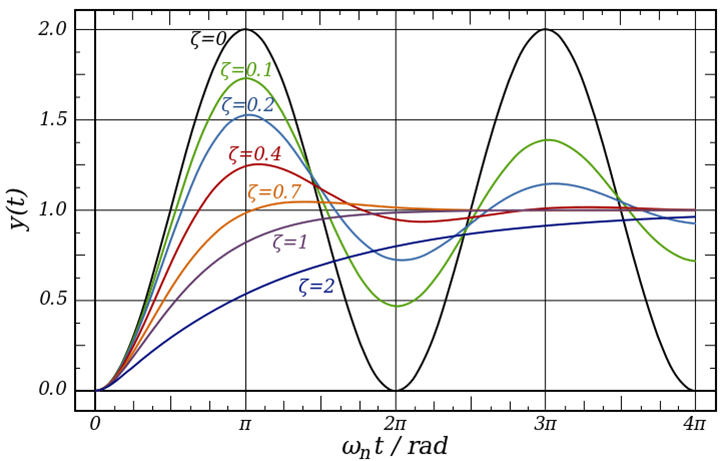
\includegraphics[width=0.8\linewidth]{Afbeelding6}
\end{itemize}
\end{frame}

\begin{frame}
\frametitle{Second order systems - characteristics}
\begin{itemize}
\item Overshoot: Highest amplitude above steady state.
\item Rise Time: Time needed to reach the steady state for the first time.
\item Peak Time: Time to reach overshoot.
\\ \begin{figure}
\centering{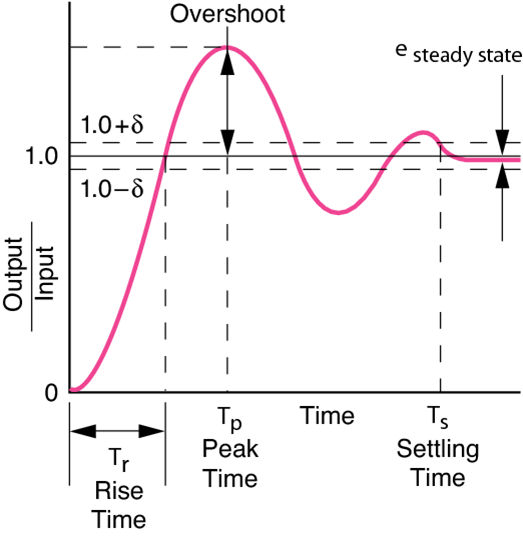
\includegraphics[width=0.45\linewidth]{Afbeelding7}}
\end{figure}
\end{itemize}
\end{frame}

\begin{frame}
\frametitle{Second order systems - characteristics}
\begin{itemize}
\item Settling Time: Time needed to approximate the steady state.
\item For: $\delta = \frac{0.02}{\sqrt{1-\zeta^2}}$
\item We find:
\vspace{-0.55cm}
\begin{align*}
 e^{-\zeta\omega_n\tau_s} &< 0.02
\\\tau_s &= \frac{4}{\omega_n\zeta}
\end{align*}
\\ \begin{figure}
\centering{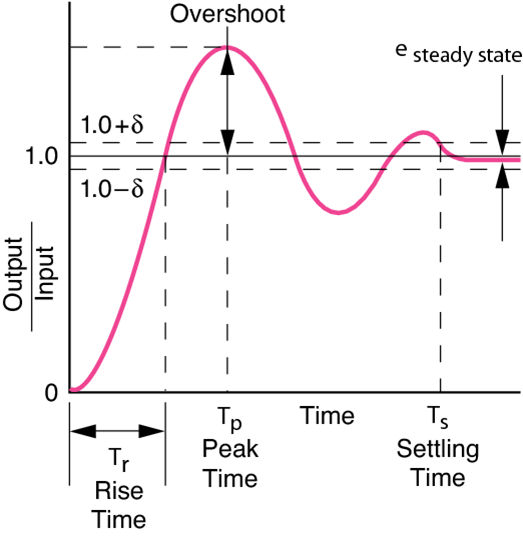
\includegraphics[width=0.45\linewidth]{Afbeelding7}}
\end{figure}
\end{itemize}
\end{frame}

\begin{frame}
\frametitle{Second order systems - resonace}
\begin{itemize}
\item The resonance frequency is the frequency at which the systems output has a larger amplitude than at other frequencies. This happens when underdamped functions oscillate at a greater magnitude than the input.
\item An input with this frequency can sometime have catastrophic effects.
\item A different view on the Tacoma bridge disaster: \url{https://www.youtube.com/watch?v=6ai2QFxStxo}
\item In fact the collapse was a result of a number of effects like Aerodynamic flutter and vortices. Read the full article here: \url{http://www.ketchum.org/billah/Billah-Scanlan.pdf}
\end{itemize}
\end{frame}

\begin{frame}
\frametitle{Second order systems - resonance}
\begin{itemize}
\item The resonance frequency is: $\omega_r = \omega_n\sqrt{1-\zeta^2}$
\item Systems with a damping $>0.707$ do not resonate
\item The resonance frequency and the natural frequency are equal when a system has no damping.
\item Another phenomenon with bridges and resonance is that many people marching with the same rhythm can cause a bridge to start resonating like the Angers bridge in $1850$. A more recent example is the Millennium bridge in London who started resonating (see video lecture 2).
\end{itemize}
\end{frame}

\begin{frame}
\frametitle{Second order systems - damping}
\begin{itemize}
\item When we want a system with no resonance, we choose one with damping $<0.707$. This means a pole between $135^{\circ}$ and $225^{\circ}$:
\\ $arctan(\frac{\sqrt{1-\zeta^2}}{\zeta}) = +135^{\circ}$
\item We mostly want a short settling time ($<4$s). This results in another restriction on the poles of the system: 
\\ \begin{aligned}
\tau_n= \frac{4}{\omega\zeta}&< 4\text{s}
\\ \omega_n\zeta&>1
\end{aligned}
\end{itemize}
\end{frame}

\begin{frame}
\frametitle{Second order systems - damping}
\begin{figure}
\centering{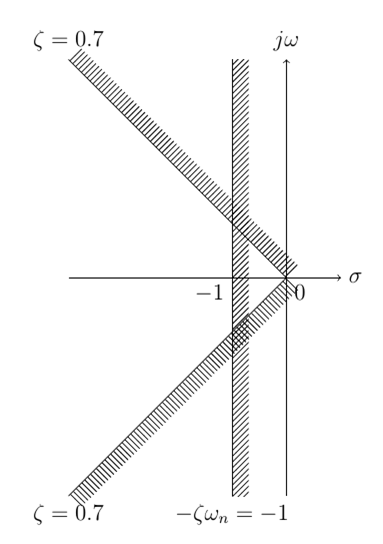
\includegraphics[width=0.5\linewidth]{Afbeelding8}}
\end{figure}
\end{frame}


